\chapter{Aplicações de Transformações Lineares}
As TL têm contribuições significativas para o campo da AL. \cite{strang2010}, renomado matemático e professor do MIT - Massachusetts Institute of Technology, aborda, por exemplo, o processamento de sinais e imagens para compressão, filtragem, reconstrução e análise de dados, a análise de redes e sistemas dinâmicos da engenharia elétrica e ciência da computação, a geometria e a computação gráfica para manipular objetos em espaços tridimensionais, videogames e modelagem em três dimensões, além de cripto segurança e, mais recentemente, análise de dados em decisões gerenciais e aprendizagem de máquina. \nocite{pitombeira1971}

A seguir, baseando em um estudo desenvolvido na Universidade Federal de Alagoas \cite{sirlandro2017}, apresentamos algumas aplicações das TL na área de engenharia.

\section{Circuitos Elétricos}
Um circuito elétrico é composto por geradores que criam correntes elétricas com magnitudes limitadas pelos resistores posicionados em série ou em paralelo, exemplificado na figura 12. Existem três unidades básicas da física: potencial elétrico $\mathbf{V}$(volts = $\mathbf{V}$), resistência elétrica $\mathbf{R}$(ohms = $\omega$) e corrente elétrica $\mathbf{I}$(ampères = $\mathbf{A}$), ), como por exemplo, baterias, que mantêm a diferença de potencial constante entre seus dois terminais.

\begin{figure}[H]
	\centering
	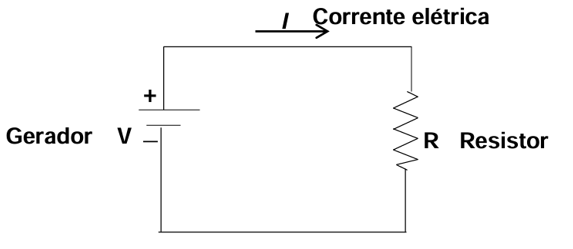
\includegraphics[scale=0.90]{a_fg1.png}
	\caption{Retirado de \cite{sirlandro2017}}
\end{figure}

Para a montagem ou avaliação de um circuito, é necessário descobrir qual a corrente elétrica que passa em cada trecho do circuito e as quedas de potencial. Dependendo do fluxo da corrente elétrica, as intensidades de corrente e as quedas de tensão podem ser positivas ou negativas. Três princípios básicos devem ser considerados:

\begin{itemize}
	\item \textbf{Lei de Ohm:} A diferença de potencial medida através de um resistor é o produto da corrente que passa por ele e a sua resistência, representado por
	
	\centerline{$\mathbf{V} = \mathbf{R} \times \mathbf{I}$},
	onde $\mathbf{V}$ é a tensão, em Volts($\mathbf{V}$, $\mathbf{R}$ é a resistência, em ohm($\omega$) e $\mathbf{I}$ é a corrente, em ampère($\mathbf{A}$).
	
	\item \textbf{Lei da corrente de Kirchhoff:} Se houver um ponto de ramificação, junção ou nó, a corrente pode se dividir e a soma das correntes que chegam no nó devem ser iguais à soma das correntes que saem do nó, representado por
	
	\centerline{$\mathbf{I} = \mathbf{I}_1 + \mathbf{I}_2$}
	
	\item \textbf{Lei das malhas ou Lei de Voltagem de Kirchhoff:} A soma algébrica das variações no potencial ao longo de qualquer malha fechada deve ser igual a zero. Para exemplificar a aplicação das leis, considera-se o circuito da figura
	
	\begin{figure}[H]
		\centering
		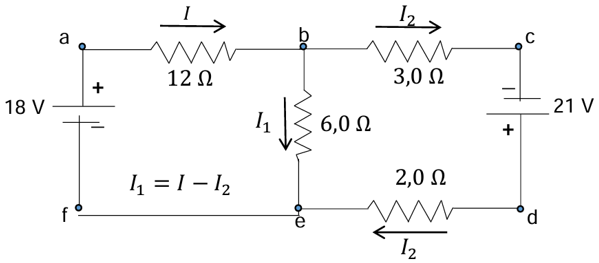
\includegraphics[scale=0.90]{a_fg2.png}
		\caption{Retirado de \cite{sirlandro2017}}
	\end{figure}
\end{itemize}

\textbf{Economia e finanças:} Nesta área as transformações lineares são aplicadas para descrever e analisar as relações entre variáveis econômicas, como oferta e demanda, investimentos e retornos financeiros. Elas são usadas em modelos de regressão linear, análise de séries temporais e precificação de ativos financeiros. \nocite{figueiredo2009}

\textbf{Engenharia e física:} Na engenharia e física, as transformações lineares são fundamentais para descrever sistemas físicos e resolver problemas de engenharia. Elas são usadas em mecânica para representar sistemas de equações diferenciais lineares que descrevem o movimento de corpos sólidos e fluidos, em eletrônica para modelar circuitos elétricos lineares e em controle de sistemas para projetar controladores lineares.

No exemplo abaixo foi selecionado a área de engenharia em análise de estruturas estáticas, no qual calcula a força em cada membro que compõe a estrutura, no caso das treliças que será o caso analise temos barras e juntas.
 
Em análise de estruturas estáticas, uma aplicação comum de transformação linear é na resolução de sistemas de equações lineares para determinar as forças internas e externas em cada membro da estrutura.

Por exemplo, considere uma treliça, que é uma estrutura composta por membros retos ligados por juntas. Para analisar as forças em cada membro da treliça sob diferentes condições de carga, pode-se usar transformações lineares para representar as forças em cada membro em termos de forças externas aplicadas e das reações nas juntas.
 
Ao formular as equações de equilíbrio para a estrutura, elas podem ser representadas como um sistema de equações lineares. A aplicação de técnicas de álgebra linear, como métodos de matriz e transformações, permite resolver eficientemente esses sistemas e determinar as forças em cada membro da treliça. Essa análise é crucial para garantir que a estrutura seja segura e capaz de suportar as cargas esperadas.
	Suponha que temos uma treliça simples com três membros e quatro nós, como mostrado abaixo:

   1
  / \
 /   \
2-----3

Podemos atribuir forças desconhecidas em cada membro da treliça (F1, F2, F3) e forças de reação nas juntas (R1x, R1y, R3x, R3y). Podemos então escrever as equações de equilíbrio para cada nó:

Para o nó 1:

$\sigma Fx = R1x - F1 = 0$
$\sigma Fy = R1y = 0$
Para o nó 2:

$\sigma Fx = -F1 = 0$
$\sigma Fy = -F2 = 0$
Para o nó 3:

$\sigma Fx = -R3x + F1 = 0$
$\sigma Fy = R3y - F3 = 0$

Além disso, podemos ter equações de equilíbrio global, como a soma das forças horizontais e verticais igual a zero.

Essas equações formam um sistema de equações lineares que pode ser representado na forma matricial Ax = b, onde A é a matriz de coeficientes, x é o vetor de incógnitas (neste caso, as forças em cada membro e as reações nas juntas) e b é o vetor de termos constantes (neste caso, zeros devido ao equilíbrio).

	Ao resolver esse sistema linear, podemos determinar as forças em cada membro da treliça e as reações nas juntas, o que nos permite analisar a estabilidade e a integridade estrutural da treliça.






 
